\chapter{RESULTS AND DISCUSSION}
\label{chap:resultsandiscussion}

% Ubah bagian-bagian berikut dengan isi dari pengujian dan analisis

This section discusses and shows the results from our test and analysis on training humanoid robot model, human model comparison, and also compares their suitability.
All tests were conducted using the Ichiro robot in the \emph{Robot Cerdas} Laboratory with computer specifications as can be seen in Table \ref{tb:computerspecichiro}.

\begin{longtable}{|c|c|}
  \caption{Computer specification on Ichiro robot.}
  \label{tb:computerspecichiro}\\
  \hline
  OS      & Ubuntu 20.04.2 LTS \\
  \hline
  CPU     & Intel i5-10210U (8) @ 4.200GHz \\
  \hline
  GPU     & Intel UHD Graphics  \\
  \hline
  RAM     & 3636 MiB \\
  \hline
\end{longtable}

\section{Robot's Model Training Result}
\label{sec:robotmodeltrainingresult}

This section shows the evaluation metrics about three models and testing we perform such as visualizing detection results and inference time.
For the evaluation metrics, We use the Object Keypoint Similarity (OKS) with a per-keypoint constant that controls fall off is equal to 0.4.
From Table \ref{tb:robotmodelcomparison} it can be seen that RCNN has the highest evaluation metric among the other models.
Moreover, RCNN showed the best detection results as shown in Table \ref{tb:robotmodelcomparisondetectionresults}, followed by NimbRo and YOLO-pose.
Lastly, Nimbro is the most likely to be applied to real-time systems because it has the lowest inference time.
However, since our main program uses the web for interaction and during PLAY mode, there is a considerable delay due to transferring two image data from the server to the client.
We decide to store the images first and do pose comparisons afterwards,
therefore we are more concerned with a reliable model than a faster model, so the RCNN model is suitable for this.

\begin{longtable}{|c|c|c|c|c|c|c|c|c|c|c|}
  \caption{Robot Model Comparison.}
  \label{tb:robotmodelcomparison}\\
  \hline
  \rowcolor[HTML]{C0C0C0}
  \textbf{Model} & \textbf{AP} & \textbf{AP\textsubscript{50}} & \textbf{AP\textsubscript{75}} & \textbf{AP\textsubscript{M}} & \textbf{AP\textsubscript{L}} & \textbf{AR} & \textbf{AR\textsubscript{50}} & \textbf{AR\textsubscript{75}} & \textbf{AR\textsubscript{M}} & \textbf{AR\textsubscript{L}} \\
  \hline
  NimbRo         & 0.828       & 0.879                         & 0.840                         & 0.886                        & 0.864                        & 0.836       & 0.884                         & 0.849                         & 0.895                        & 0.872 \\
  \hline                        
  RCNN           & 0.879       & 0.936                         & 0.904                         & 0.859                        & 0.937                        & 0.925       & 0.973                         & 0.944                         & 0.936                        & 0.955 \\
  \hline                        
  YOLO           & 0.849       & 0.838                         & -                             & -                            & -                            & 0.814       & -                             & -                             & -                            & - \\
  \hline
\end{longtable}

\begin{longtable}{|c|c|c|}
  \caption{Robot Model Comparison Detection Results.}
  \label{tb:robotmodelcomparisondetectionresults}\\
  \hline
  \rowcolor[HTML]{C0C0C0}
  \textbf{NimbRo}    & \textbf{RCNN} & \textbf{YOLO-pose}\\
  \hline
  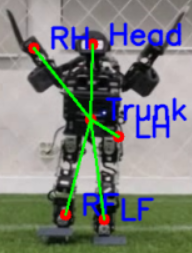
\includegraphics{gambar/nimbro-1.png} & 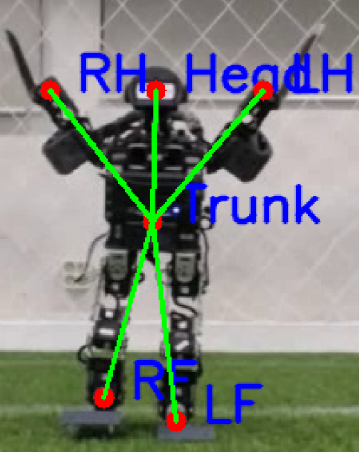
\includegraphics{gambar/rcnn-1.png} & 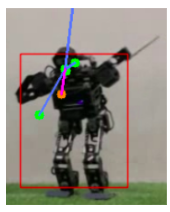
\includegraphics{gambar/yolo-1.png} \\
  \hline
  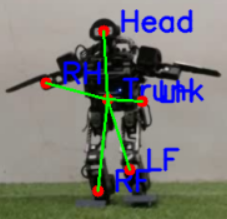
\includegraphics{gambar/nimbro-2.png} & 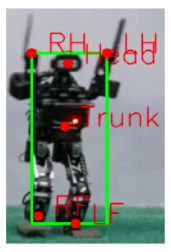
\includegraphics{gambar/rcnn-2.png} & 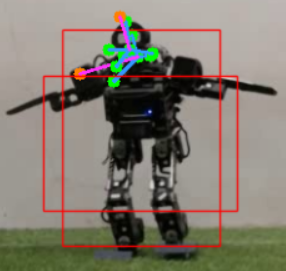
\includegraphics{gambar/yolo-2.png} \\
  \hline
  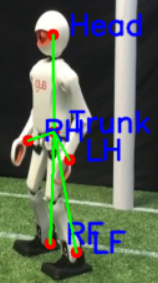
\includegraphics{gambar/nimbro-3.png} & 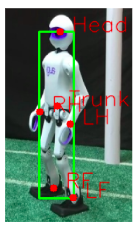
\includegraphics{gambar/rcnn-3.png} & 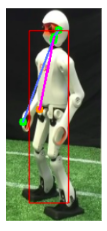
\includegraphics{gambar/yolo-3.png} \\
  \hline
\end{longtable}

\begin{longtable}{|c|c|c|}
  \caption{Inference Time Model Humanoid Robot.}
  \label{tb:inferencerobot}\\
  \hline
  \rowcolor[HTML]{C0C0C0}
  \textbf{Model}    & \textbf{PyTorch (s)} & \textbf{OpenVINO (s)}\\
  \hline
  NimbRo's Model & 0.4 - 0.5 & 0.15 - 0.2 \\
  \hline
  RCNN Keypoint   & 3.5 - 4.0 & 1.25 \\
  \hline
  YOLO-pose   &  &  \\
  \hline
\end{longtable}


\section{Human's Model Comparison}
\label{sec:humanmodelcomparison}

Based on \parencite{bazarevsky2020} that compares three different models: BlazePose Lite, BlazePose Full, and OpenPose (body only), they test the models on AR Dataset and Yoga Dataset. As an evaluation metric, they use the Percent of Correct Points with 20\% tolerance (PCK@0.2)
(where assuming the point to be detected correctly if the 2D Euclidian error is smaller than 20\% of the corresponding person's torso size). BlazePose shows slightly worse performance than the OpenPose model on the AR dataset but BlazePose Full outperforms OpenPose on Yoga/Fitness use cases.
Note that, in this study, we use BlazePose Full because by default the value of \emph{model complexity} argument is 1 in the \emph{mediapipe.solutions.pose.Pose} API class. Mediapipe provides 3 BlazePose models: BlazePose Lite, BlazePose Full, and BlazePose Heavy. Pose landmark accuracy as well as inference latency generally go up with the model complexity.
Table \ref{tb:yoloandmediapipecomparison} shows the comparison between YOLO-pose and MediaPipe Pose and based on our needs to just detect one person, MediaPipe should be the best and also reliable choice.  

\begin{longtable}{|p{3cm}|p{5cm}|p{5cm}|}
  \caption{YOLO-pose and MediaPipe Pose Comparison.}
  \label{tb:yoloandmediapipecomparison}\\
  \hline
  \rowcolor[HTML]{C0C0C0}
  \textbf{Features}    & \textbf{YOLO-pose} & \textbf{MediaPipe Pose}\\
  \hline
  Topology             & 17 Keypoints COCO  & 33 Keypoints COCO \\
  \hline
  Workflow             & Detection runs for all frames & Detection runs once followed by tracker until occlusion occurs \\
  \hline
  GPU support          & Support for both CPU and GPU & Only CPU \\
  \hline
  Number of persons    & Multi-person & Single person \\
  \hline
\end{longtable}

\begin{longtable}{|c|c|c|}
  \caption{Inference Time Model Human.}
  \label{tb:inferencehuman}\\
  \hline
  \rowcolor[HTML]{C0C0C0}
  \textbf{Model}    & \textbf{PyTorch (s)} & \textbf{OpenVINO (s)}\\
  \hline
  OpenPose    &  &  \\
  \hline
  Mediapipe   &  &  \\
  \hline
  YOLO-Pose   &  &  \\
  \hline
\end{longtable}

\section{Comparing the Suitability Between Humanoid Robot Pose and Human Pose Results}
\label{sec:comparingsuitabilityresults}
